\section{Additional Results}
\label{app:results}

\begin{table}[H]
    \centering
    \small
    \begin{tabular}{@{}lcccccc@{}}
        \toprule
        \textbf{Setting} & \textbf{point} & \textbf{uniform} & \textbf{normal} & \textbf{Laplace} & \textbf{$t_3$} & \textbf{\lnhard} \\
        \midrule
        Base (SD $= 1.5$, $\Nitems = 500$) & 7.3 & {\bf 9.0} & {\bf 9.0} & 8.9 & 8.5 & 8.2 \\
        SD $= 3.0$                         & 7.3 & {\bf 12.5} & 12.3 & 11.3 & 10.4 & 9.2 \\
        $\Nitems = 100$                    & 3.5 & {\bf 4.3} & 4.0 & 3.8 & 3.8 & 3.6 \\
        \bottomrule
    \end{tabular}
    \caption{{\bf Effective lifetime in the IRT model} (logits of frontier ability with $\rho \ge 0.5$). Longest lifetime per row in {\bf bold}. Uniform has the longest lifetime among matched-variance shapes; the heavy hard tail is shorter. The point mass does not depend on SD.}
    \label{tab:lifetime_app}
\end{table}

\begin{table}[H]
    \centering
    \small
    \begin{tabular}{@{}lcccc@{}}
        \toprule
        \textbf{Items} & 50 & 100 & 200 & 500 \\
        \midrule
        Seed share (greedy) & 0.51 & 0.45 & 0.32 & 0.18 \\
        \bottomrule
    \end{tabular}
    \caption{{\bf Seed share \versus benchmark size} for the \arce top-6 cohort (96\% accuracy). Seed noise dominates only at 50 items.}
    \label{tab:nitems}
\end{table}

\begin{figure}[H]
    \centering
    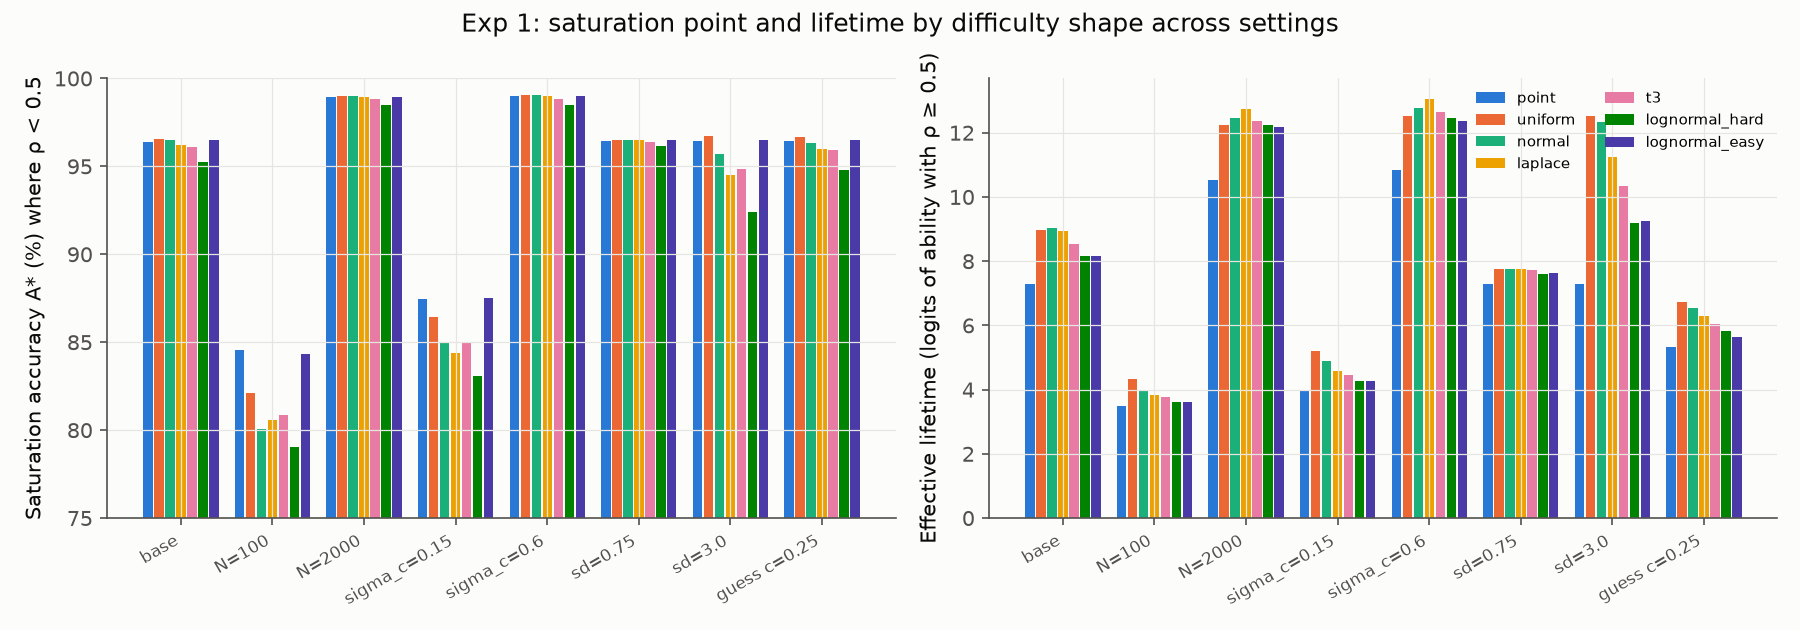
\includegraphics[width=0.95\linewidth]{figures/exp1_shape_settings.png}
    \caption{{\bf Saturation accuracy $\astar$ \figleft{} and effective lifetime \figright{} for each difficulty shape across sensitivity settings} of the IRT model. Within each setting, bars differ little in $\astar$; across settings, item count ($\Nitems$) and cohort spread ($\sigc$) produce the large changes.}
    \label{fig:exp1_settings}
\end{figure}

\begin{figure}[H]
    \centering
    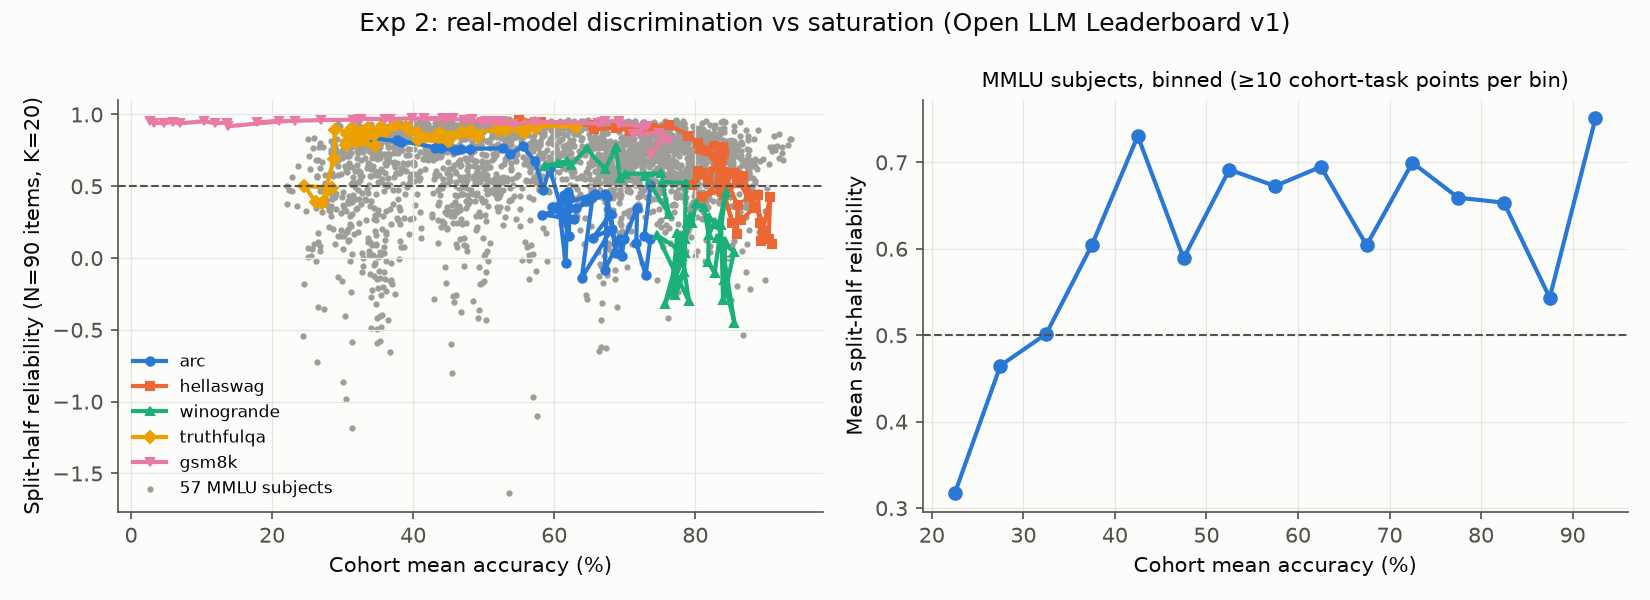
\includegraphics[width=0.95\linewidth]{figures/exp2_reliability_vs_accuracy.png}
    \caption{{\bf Real-model discrimination \versus cohort accuracy} (\leaderboard, 20-model cohorts, 90-item subsamples). \figleft{} Split-half reliability per task; grey points are the 57 \mmlu subjects. \hellaswag and \winogrande lose discrimination for the top cohorts, while \gsm and \truthfulqa stay reliable. \figright{} Mean reliability of \mmlu subjects binned by accuracy; it does not decline toward high accuracy over the observed range.}
    \label{fig:exp2_reliability}
\end{figure}

\section{Experimental Details}
\label{app:details}

\para{IRT model (Exp~1).} Discriminations $a_i \sim \mathrm{LogNormal}(0, 0.3^2)$. Difficulty shapes are rescaled to the target SD and centred. The cohort centre is swept over 221 ability levels; accuracy mean and variance are computed exactly with the Poisson-binomial distribution. Kendall $\tau$ uses 200 Monte Carlo replicates per level. Each shape is replicated over 20 independent item draws.

\para{Leaderboard data (Exp~2, Exp~4).} Data come from the public \texttt{open-llm-leaderboard-old} details and contents datasets. Of 245 sampled models, 227 had at least 60 of 62 tasks and 220 had all 62. Metrics: \arcc acc\_norm (25-shot), \hellaswag acc\_norm (10-shot), \truthfulqa mc1 (0-shot), \winogrande acc (5-shot), \gsm exact match (5-shot), \mmlu acc (5-shot). The Rasch fit uses joint MAP estimation with L-BFGS in PyTorch.

\para{Seed evaluation (Exp~3).} Items: 500 test items each from \arce, \arcc~\citep{clark2018think} and \mmlu~\citep{hendrycks2021measuring}, sampled with seed 42. Models were run in bf16 with Hugging Face \texttt{transformers}. Seed 0 uses the original option order; seeds 1--9 apply random permutations. The answer distribution is the next-token probability over letters A--D after the prefix ``The answer is'', renormalised. Total: 15 models $\times$ 1{,}500 items $\times$ 10 seeds $= 225{,}000$ forward passes.
